\section{Methodology}\label{sec:methodology}

Th problem defined in section \ref{sec:model_overview} describes a normal-form
game between the decision makers of two queueing systems and a third player that 
decides how to distribute individuals to the systems.
The strategy space of the two queueing systems is defined as the possible values
that the threshold parameter can take \(T_i \in (1, N_i)\).
Then, the distributor has to decide on the proportion of individuals to send to 
each queueing system \(p_A \text{ and } p_B\), where \(p_A, p_B \in [0, 1] \)
and \(p_A + p_B = 1\).
Figure \ref{fig:imperfect-info-game} shows a diagrammatic 
representation of the game to be played and the decisions to be made.

\begin{figure}[ht]
    \centering
    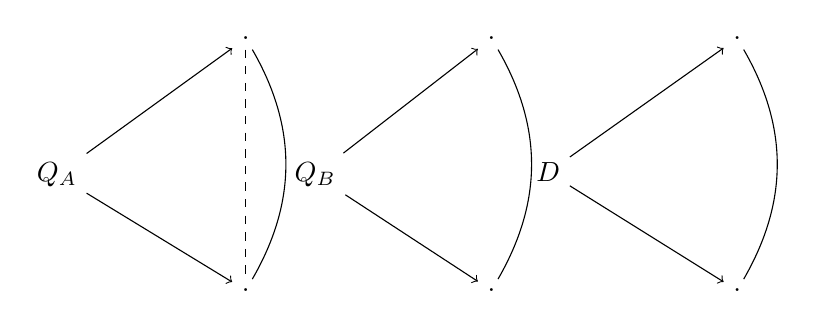
\begin{tikzpicture}[-, node distance = 3cm, scale=0.8]
        \node[anchor=north](HA){\(Q_A\)};
        \node[anchor=north](HA_d1) at (3, 2){.};
        \node[anchor=north](HA_d2) at (3, -2){.};
    
        \path[->] (HA) edge node {}(HA_d1);
        \path[->] (HA) edge node {}(HA_d2);
        \path (HA_d1) edge [bend left] node {}(HA_d2);
        \path (HA_d1) [dashed] edge node {}(HA_d2);
    
        \node[anchor=north](HB) at (4.1, 0){\(Q_B\)};
        \node[anchor=north](HB_d1) at (6.9, 2){.};
        \node[anchor=north](HB_d2) at (6.9, -2){.};
    
        \path[->] (HB) edge node {}(HB_d1);
        \path[->] (HB) edge node {}(HB_d2);
        \path(HB_d1) edge [bend left] node {}(HB_d2);
    
        \node[anchor=north](D) at (7.8, 0){\(D\)};
        \node[anchor=north](D_d1) at (10.8, 2){.};
        \node[anchor=north](D_d2) at (10.8, -2){.};
        
        \path[->] (D) edge node {}(D_d1);
        \path[->] (D) edge node {}(D_d2);
        \path(D_d1) edge [bend left] node {}(D_d2);
    \end{tikzpicture}
    \caption*{Figure 2 (revisited): Imperfect information Extensive Form Game 
    between the distributor and the 2 queueing systems}
\end{figure}

As described in section \ref{sec:model_overview} queueing system \(A\) decides
on a strategy, then queueing system \(B\) chooses its own threshold, unaware 
of the first queueing system's choice.
Finally, the distributor makes its choice based on the strategies that the 
queueing systems chose to play. 

The problem can be formulated by 3 matrices; the two payoff matrices of the 
normal form game and the routing matrix.
The payoff matrices and their utilities are defined by equations 
(\ref{eq:payoff-entry}) and (\ref{eq:payoff_matrices}) is section 
\ref{sec:model_overview}:

\begin{equation*}
    A = 
    \begin{pmatrix}
        U_{1,1}^A & U_{1,2}^A & \dots & U_{1,N_B}^A \\
        U_{2,1}^A & U_{2,2}^A & \dots & U_{2,N_B}^A \\
        \vdots & \vdots & \ddots & \vdots \\
        U_{N_A,1}^A & U_{N_A,2}^A & \dots & U_{N_A,N_B}^A \\
    \end{pmatrix},
    B = 
    \begin{pmatrix}
        U_{1,1}^B & U_{1,2}^B & \dots & U_{1,N_B}^B \\
        U_{2,1}^B & U_{2,2}^B & \dots & U_{2,N_B}^B \\
        \vdots & \vdots & \ddots & \vdots \\
        U_{N_A,1}^B & U_{N_A,2}^B & \dots & U_{N_A,N_B}^B \\
    \end{pmatrix}
    \tag{\ref{eq:payoff_matrices} revisited}
\end{equation*}


Similarly, the entries of the routing matrix are defined by equation 
(\ref{eq:obj_distributor}):
\begin{equation*}
    p_A, p_B \quad s.t. \quad \alpha P(L_A) + (1 - \alpha) B_A = \alpha P(L_B) 
    + (1 - \alpha) B_B \tag{\ref{eq:obj_distributor} revisited}
\end{equation*}

Equation \ref{eq:obj_distributor} is properly defined and explained in section 
\ref{sec:model_overview}.
Thus, using equation \ref{eq:obj_distributor} for all possible sets of 
thresholds we can get the full routing matrix that consists of the proportions
to send to queueing system A (\(p_A\)) and to queueing system B (\(p_B\)).

\begin{equation}\label{eq:routing_matrix}
    R_A = 
    \begin{pmatrix}
        (p_{1,1}^A, p_{1,1}^B) & (p_{1,2}^A, p_{1,2}^B) & \dots & 
        (p_{1,N_B}^A, p_{1,N_B}^B) \\
        (p_{2,1}^A, p_{2,1}^B) & (p_{2,2}^A, p_{2,2}^B) & \dots & 
        (p_{2,N_B}^A, p_{2,N_B}^B) \\
        \vdots & \vdots & \ddots & \vdots \\
        (p_{N_A,1}^A, p_{N_A,1}^B) & (p_{N_A,2}^A, p_{N_A,2}^B) & \dots & 
        (p_{N_A,N_B}^A, p_{N_A,N_B}^B) \\
    \end{pmatrix}
\end{equation}

The game can thus be partitioned into a normal form game between the
two queueing systems and then finding the distributor's best strategy. 

\subsection{Backwards Induction}

\subsection{Nash Equilibrium}

\subsection{Learning Algorithms}
